\section{Typologie des bases\\de données NoSQL}

\begin{frame}{Ecosystème NoSQL}
    \begin{figure}[htb]
        \centering
        \resizebox{0.95\textwidth}{!}{
        \begin{tikzpicture}
            \node[minimum width=3cm, minimum height=2cm] at (0, 0) {\includesvg[height=1cm]{img/db/redis.svg}};
            \node[minimum width=3cm, minimum height=2cm] at (1.5, -1) {
\includegraphics[height=0.8cm]{img/db/oracle-nosql.png}};
            \node[minimum width=3cm, minimum height=2cm] at (4, -0.5) {\includesvg[height=1cm]{img/db/couchdb.svg}};
            \node[minimum width=3cm, minimum height=2cm] at (6, 0.2) {\includesvg[height=1.3cm]{img/db/aws-documentdb.svg}};
            \node[minimum width=3cm, minimum height=2cm] at (0, -2) {\includesvg[height=0.8cm]{img/db/couchbase.svg}};
            \node[minimum width=3cm, minimum height=2cm] at (0.5, -6) {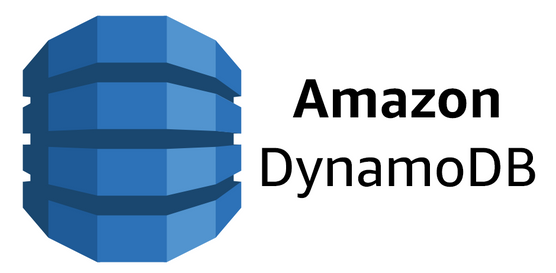
\includegraphics[height=1cm]{img/db/aws-dynamodb.png}};
            \node[minimum width=3cm, minimum height=2cm] at (2, -3.5) {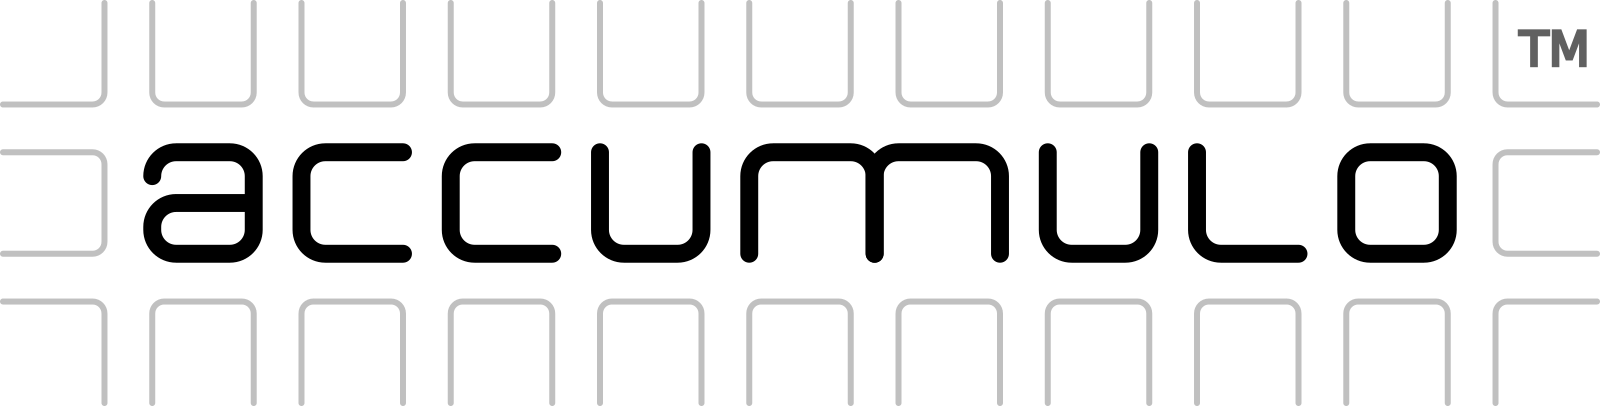
\includegraphics[height=1cm]{img/db/accumulo.png}};
            \node[minimum width=3cm, minimum height=2cm] at (2, -4.8) {\includesvg[height=1cm]{img/db/mongodb.svg}};
            \node[minimum width=3cm, minimum height=2cm] at (4.5, -4.8) {
\includegraphics[height=1.2cm]{img/db/scylla-db.png}};
            \node[minimum width=3cm, minimum height=2cm] at (6, -2) {\includesvg[height=0.6cm]{img/db/ravendb.svg}};
            \node[minimum width=3cm, minimum height=2cm] at (-1.5, -3.2) {
\includegraphics[height=1cm]{img/db/hypertable.png}};
            \node[minimum width=3cm, minimum height=2cm] at (7.5, -5.5) {\includesvg[height=1cm]{img/db/firestore.svg}};
            \node[minimum width=3cm, minimum height=2cm] at (3, -2.3) {\includesvg[height=0.7cm]{img/db/riak.svg}};
            \node[minimum width=3cm, minimum height=2cm] at (-2, -6) {\includesvg[height=1cm]{img/db/cassandra.svg}};
            \node[minimum width=3cm, minimum height=2cm] at (7, -4) {\includesvg[height=1cm]{img/db/hbase.svg}};
            \node[minimum width=3cm, minimum height=2cm] at (-1.5, -1) {
\includegraphics[height=0.8cm]{img/db/gcp-bigtable.png}};
            \node[minimum width=3cm, minimum height=2cm] at (3, -6) {\includesvg[height=0.7cm]{img/db/druid.svg}};
            \node[minimum width=3cm, minimum height=2cm] at (-1.3, -4.5) {\includesvg[height=1cm]{img/db/neo4j.svg}};
            \node[minimum width=3cm, minimum height=2cm] at (7, -1) {\includesvg[height=1cm]{img/db/arangodb.svg}};
            \node[minimum width=3cm, minimum height=2cm] at (7, -3) {\includesvg[height=1cm]{img/db/orientdb.svg}};
            \node[minimum width=3cm, minimum height=2cm] at (6, -5.5) {
\includegraphics[height=1.3cm]{img/db/aws-neptune.png}};
            \node[minimum width=3cm, minimum height=2cm] at (7, -7) {\includesvg[height=1cm]{img/db/memcached.svg}};
        \end{tikzpicture}
        }
    \end{figure}
\end{frame}


\begin{frame}{Typologie des bases de données NoSQL}

    \begin{figure}
        \centering
        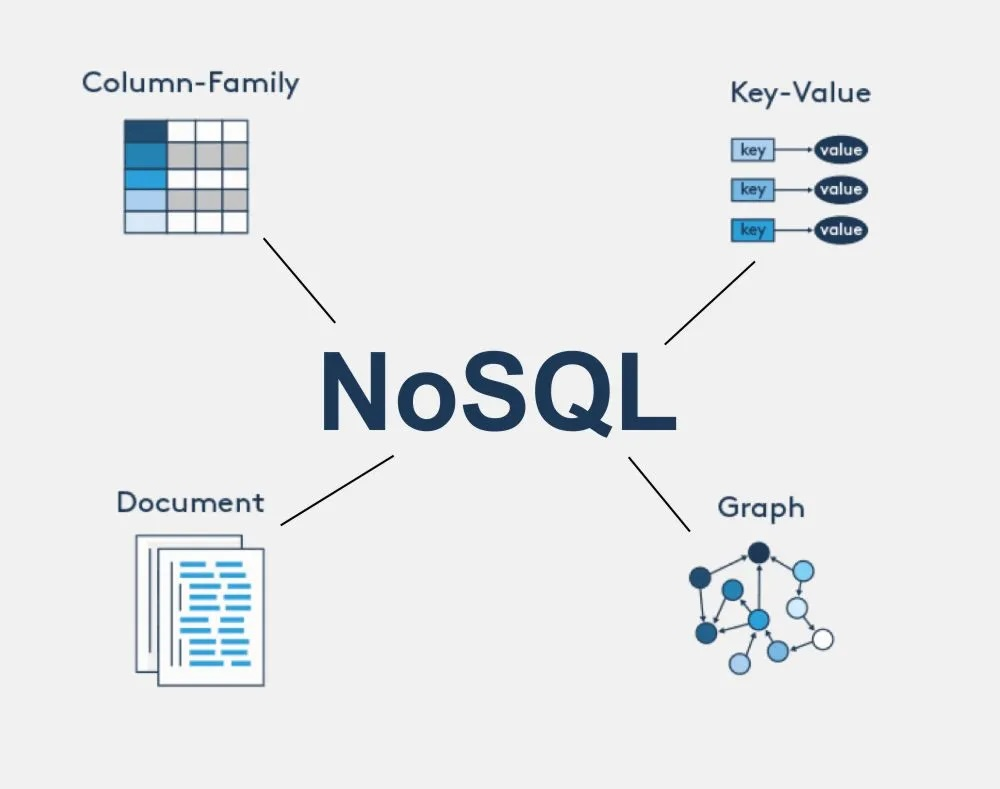
\includegraphics[width=0.8\textwidth]{img/nosql-database-types.jpg}
    \end{figure}

\end{frame}

% ------------------------------------------------------------------------------------------------------------------------------------------------------------------------

\begin{frame}[standout]

    Bases de données clé-valeur

\end{frame}

\begin{frame}
    "Une base clé-valeur, c’est comme un dictionnaire : tu cherches un mot (clé) et tu obtiens sa définition (valeur)."
\end{frame}

\begin{frame}{Caractéristiques des bases de données clé-valeur}

    \begin{definitionbox}
        Dans une base de données clé-valeur, les données sont stockées sous forme de \textbf{paires de clés uniques et de valeurs} correspondantes.

        La clé agit comme un \textbf{identifiant unique}, et la valeur peut être de tout type (chaîne de caractères, JSON, binaire, etc.).
    \end{definitionbox}

    \begin{noteblock}
        \begin{itemize}
            \item Très scalable avec une structure simple.
            \item Pas de schéma ou de structure rigide ; stockage de données flexible.
        \end{itemize}
        % $\Longrightarrow$ Idéal pour stocker de grandes quantités de données avec une complexité relationnelle minimale.
        $\hookrightarrow$ Idéal pour stocker de grandes quantités de données avec une complexité relationnelle minimale.
    \end{noteblock}
\end{frame}

\begin{frame}{Comment fonctionnent les bases de données clé-valeur ?}

    \begin{figure}
        \centering
        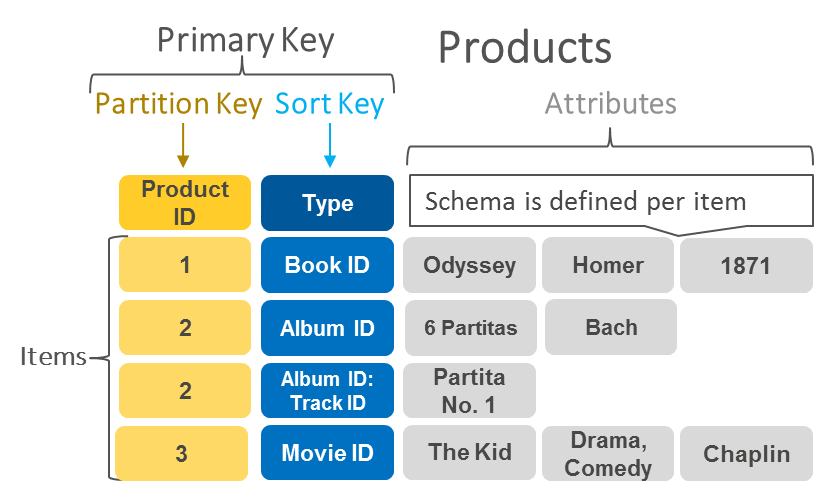
\includegraphics[width=0.8\textwidth]{img/key-value-database.png}
    \end{figure}

\end{frame}

\begin{frame}{Bases de données clé-valeur}
    \begin{figure}[htb]
        \centering
        \begin{tikzpicture}
            \node[minimum width=3cm, minimum height=2cm] at (0, 0) {\includesvg[height=1cm]{img/db/redis.svg}};
            \node[minimum width=3cm, minimum height=2cm] at (0, -2) {\includesvg[height=1cm]{img/db/riak.svg}};
            \node[minimum width=3cm, minimum height=2cm] at (4, 0) {\includesvg[height=1cm]{img/db/memcached.svg}};
            \node[minimum width=3cm, minimum height=2cm] at (4, -2) {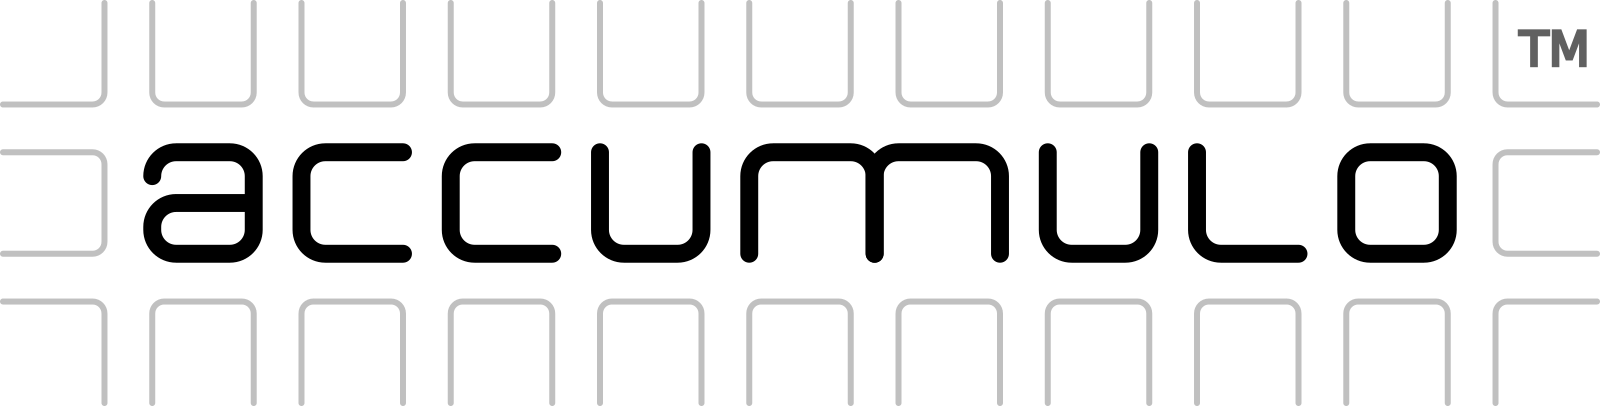
\includegraphics[height=1cm]{img/db/accumulo.png}};
            \node[minimum width=3cm, minimum height=2cm] at (0, -4) {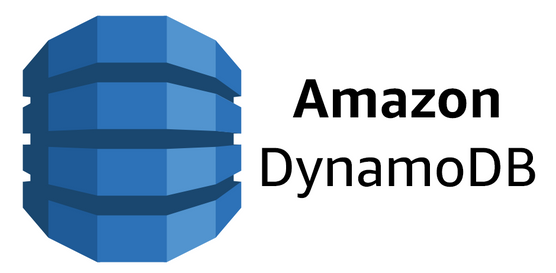
\includegraphics[height=1cm]{img/db/aws-dynamodb.png}};
            \node[minimum width=3cm, minimum height=2cm] at (4, -4) {
\includegraphics[height=1cm]{img/db/oracle-nosql.png}};
        \end{tikzpicture}
    \end{figure}
\end{frame}


\begin{frame}{Cas d'usages des bases de données clé-valeur}
    % Gestion de session
    % Une application orientée session telle qu'une application web ouvre une session lorsqu'un utilisateur se connecte à une application,
    % puis ferme la session lorsque l'utilisateur se déconnecte ou lorsque la session expire.
    % Pendant cette période, l'application stocke tous les attributs de la session utilisateur dans la mémoire principale ou dans une base de données.
    % Les données de session peuvent inclure des informations sur le profil d'utilisateur, des messages, des données et des thèmes personnalisés,
    % des recommandations, des promotions ciblées et des remises.
    % Chaque session utilisateur possède un identifiant unique. Les données de session sont uniquement interrogées par une clé primaire.
    % Ainsi, un magasin clé-valeur rapide est idéal dans ce contexte. En général, les frais généraux par page liés aux bases de données clé-valeur
    % sont inférieurs à ceux associés aux bases de données relationnelles.

    % Panier d'achat
    % Un site Web d'e-commerce peut recevoir des milliards de commandes en quelques secondes pendant la période des achats de Noël.
    % Les bases de données clé-valeur peuvent gérer la mise à l'échelle de grandes quantités de données et de grands volumes de changements d'état
    % tout en répondant aux besoins de millions d'utilisateurs simultanés grâce à un traitement et à un stockage distribués.
    % Le stockage de données clé-valeur intègre également une capacité de redondance, ce qui lui permet de gérer la perte de nœuds de stockage.

    % Moteur de stockage des métadonnées
    % Votre stockage clé-valeur peut servir de couche de stockage sous-jacente pour des niveaux d'accès aux données plus élevés.
    % Par exemple, vous pouvez mettre à l'échelle le débit et la simultanéité pour les charges de travail multimédias et de divertissement
    % telles que le streaming vidéo en temps réel et le contenu interactif. Vous pouvez également créer votre plateforme de jeu avec les données
    % des joueurs, l'historique des sessions et les tableaux de classement pour des millions d'utilisateurs simultanés.

    % Mise en cache
    % Vous pouvez utiliser une base de données clé-valeur pour stocker temporairement des données afin de les récupérer plus rapidement.
    % Par exemple, les applications de réseaux sociaux peuvent stocker des données fréquemment consultées, telles que le contenu des fils d'actualités.
    % Les systèmes de mise en cache des données en mémoire utilisent également le stockage clé-valeur pour accélérer les réponses des applications.

    \begin{itemize}
        \item \textbf{Stockage de sessions et profils d'utilisateurs}\\
        $\hookrightarrow$ Chaque utilisateur est référencé par une clé qui permet d'accéder à ses informations.
        \vspace{0.3cm}

        \item \textbf{Paniers d'achats dans les applications de commerce électronique}\\
        $\hookrightarrow$ Gestion des commandes lors des soldes et de l'évolution de leur statut.
        \vspace{0.3cm}

        \item \textbf{Moteur de stockage des métadonnées}\\
        $\hookrightarrow$ Pour une plateforme de jeu, cela permet d'accéder aux données des joueurs, l'historique des sessions et les tableaux de classement pour des millions d'utilisateurs simultanés.
        \vspace{0.3cm}

        \item \textbf{Systèmes de cache (ex. : Redis, Memcached)}\\
        $\hookrightarrow$ Les applications de réseaux sociaux peuvent stocker des données fréquemment consultées, telles que le contenu des fils d'actualités.
    \end{itemize}
\end{frame}

\begin{frame}{Avantages et inconvénients des bases de données clé-valeur}
    \vfill
    \prosbox{
        \textbf{Avantages}
        \begin{itemize}
            \item Lectures et écritures extrêmement rapides grâce à l'accès direct par clé.
            \item Scalabilité horizontale facile pour de grands ensembles de données.
        \end{itemize}
    }
    \vfill
    \pause
    \consbox{
        \textbf{Inconvénients}
        \begin{itemize}
            \item Absence de requêtes complexes.
            \item Mauvaise gestion du schéma.
        \end{itemize}
    }
    \vfill
\end{frame}


\begin{frame}{Focus sur Redis}

\end{frame}

\begin{frame}[standout]

    Bases de données document

\end{frame}

\begin{frame}{Caractéristiques des bases de données document}

    \begin{definitionbox}
        Dans une base de données orientée document, les données sont stockées sous forme de \textbf{documents} structurés, généralement au format \textbf{JSON}, \textbf{BSON}, ou \textbf{XML}.

        Chaque document représente un enregistrement, ce qui permet de stocker des données hiérarchiques et complexes.
    \end{definitionbox}

    \begin{noteblock}
        \begin{itemize}
            \item Très flexible : chaque document peut avoir une structure différente.
            \item Capable de stocker des données complexes et imbriquées.
        \end{itemize}
        $\hookrightarrow$ Idéal pour des applications nécessitant un modèle de données flexible et des mises à jour fréquentes.
    \end{noteblock}
\end{frame}

\begin{frame}{Bases de données document}
    \begin{figure}[htb]
        \centering
        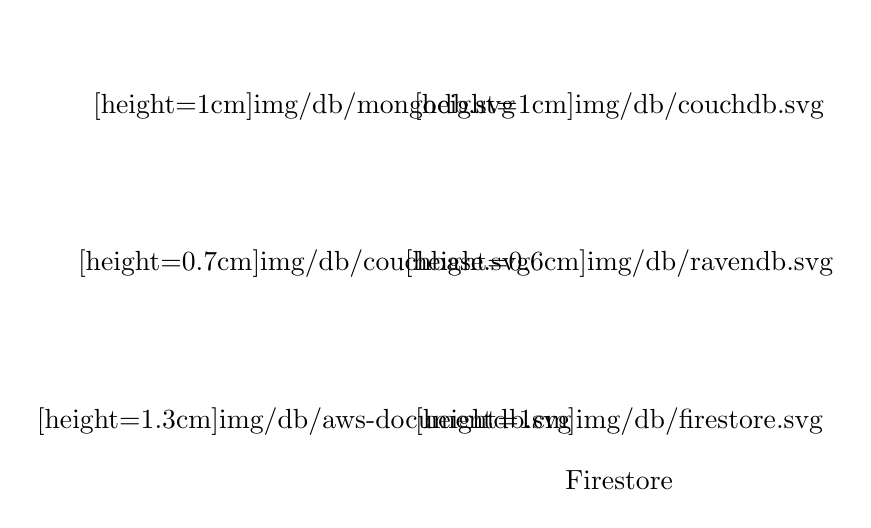
\begin{tikzpicture}
            \node[minimum width=3cm, minimum height=2cm] at (0, 0) {\includesvg[height=1cm]{img/db/mongodb.svg}};
            \node[minimum width=3cm, minimum height=2cm] at (4, 0) {\includesvg[height=1cm]{img/db/couchdb.svg}};
            \node[minimum width=3cm, minimum height=2cm] at (0, -2) {\includesvg[height=0.7cm]{img/db/couchbase.svg}};
            \node[minimum width=3cm, minimum height=2cm] at (4, -2) {\includesvg[height=0.6cm]{img/db/ravendb.svg}};
            \node[minimum width=3cm, minimum height=2cm] at (0, -4) {\includesvg[height=1.3cm]{img/db/aws-documentdb.svg}};
            \node[minimum width=3cm, minimum height=1cm,label=below:Firestore] at (4, -4) {\includesvg[height=1cm]{img/db/firestore.svg}};
        \end{tikzpicture}
    \end{figure}
\end{frame}

\begin{frame}[fragile]{Exemple de document JSON}

\begin{minted}[fontsize={\fontsize{6.7}{7.7}\selectfont}]{json}
[
    {
        "title": "Mamma Mia!",
        "year" : 2008,
        "cast" : {
            "director" : "Phyllida Lloyd",
            "actors" : ["Meryl Streep", "Pierce Brosnan","Amanda Seyfried"]
        },
        "rating" : 6.4,
        "plot" : "The story of a bride-to-be trying to find her real father told
using hit songs by the popular '70s group ABBA."
    },
    {
        "title": "Inception",
        "year" : 2010,
        "rating" : 8.8,
        "genres" : ["Action", "Adventure", "Sci-Fi"],
        "plot" : "A thief who steals corporate secrets through the use of dream-sharing
technology is given the inverse task of planting an idea into the mind of a CEO."
    }
]
\end{minted}

\end{frame}

\begin{frame}{Comment fonctionnent les bases de données document ?}

    \begin{figure}
        \centering
        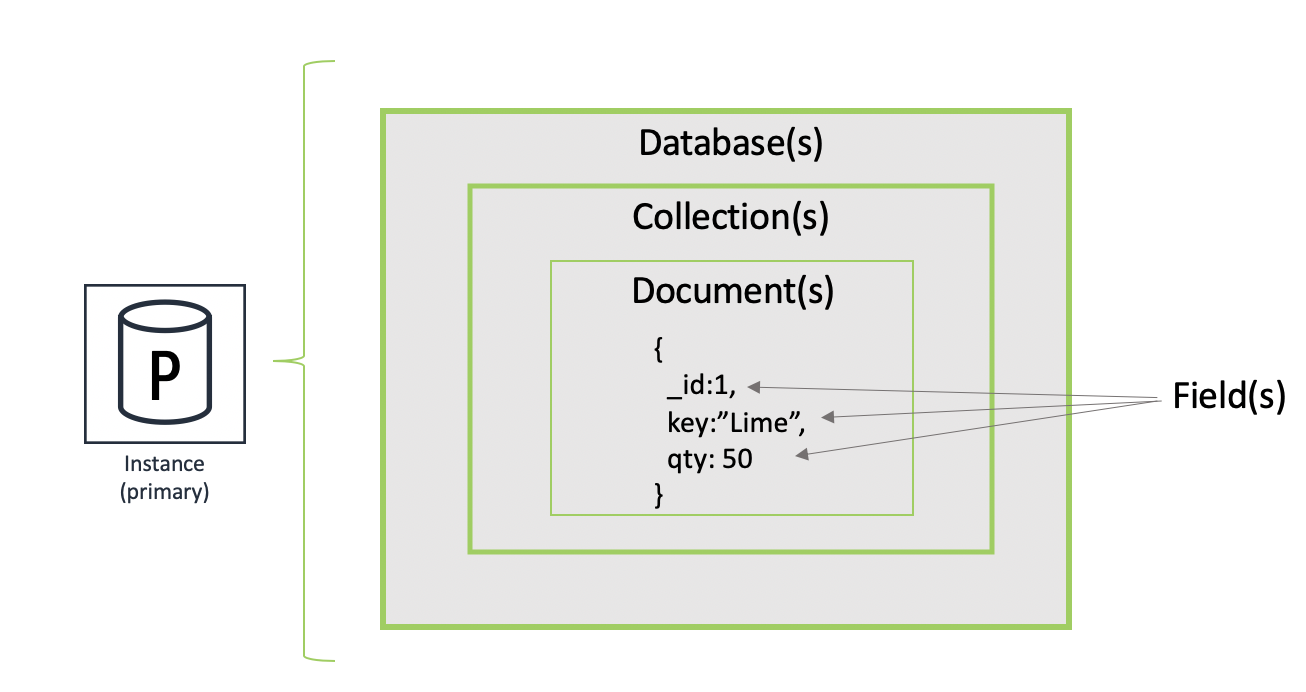
\includegraphics[width=0.8\textwidth]{img/json-document-database.png}
    \end{figure}

\end{frame}


\begin{frame}{Comment fonctionnent les bases de données document ?}

    \textbf{TODO : remplacer l'image par un filtrage sur les données de l'exemple JSON de l'exemple précédent.}

    \begin{figure}
        \centering
        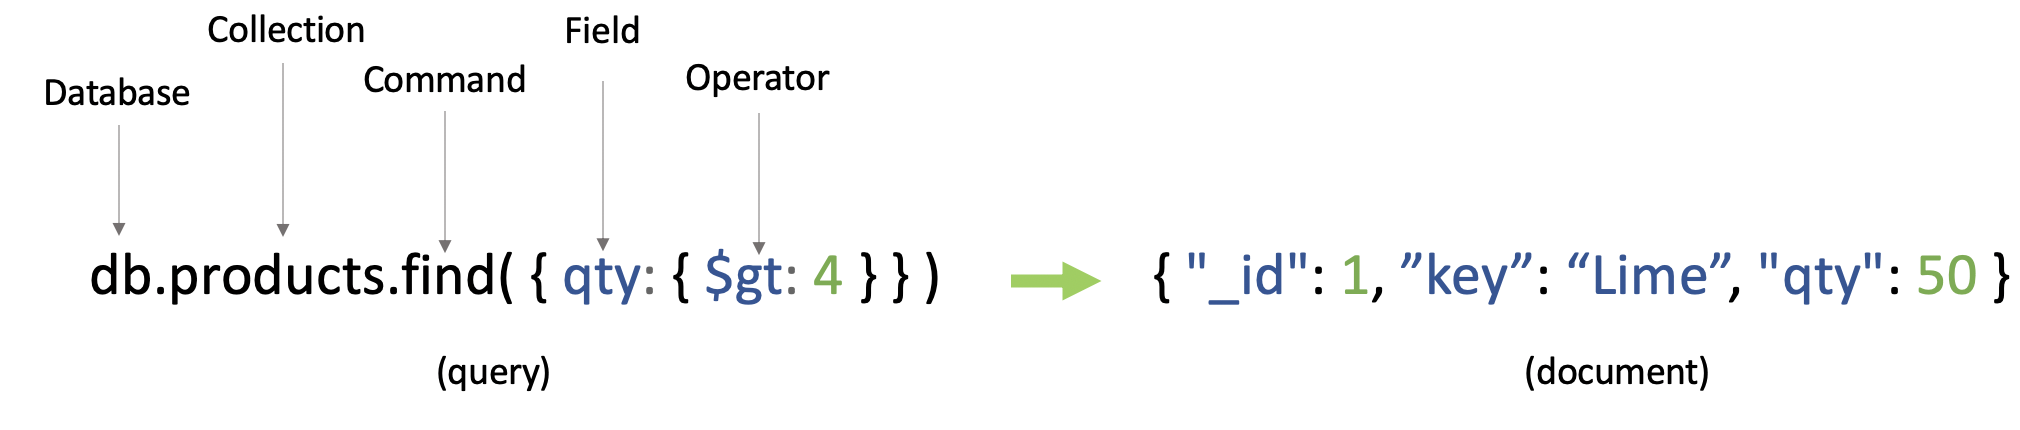
\includegraphics[width=0.8\textwidth]{img/json-database-query.png}
    \end{figure}

\end{frame}

\begin{frame}{Cas d'usages des bases de données document}

\begin{itemize}
    \item \textbf{Gestion du contenu sur les réseaux sociaux}\\
    $\hookrightarrow$ L'activité de chaque utilisateur est stockée sous forme d'un document contenant des informations imbriquées telles que les posts, commentaires, et connexions.
    \vspace{0.3cm}

    \item \textbf{Plateformes de gestion de contenu (CMS)}\\
    $\hookrightarrow$ Stockage de documents flexibles qui contiennent des informations sur des articles de blog, des images, des métadonnées, etc.
    \vspace{0.3cm}

    \item \textbf{Gestion des capteurs}\\
    $\hookrightarrow$ L'Internet des objets (IoT) permet de collecter un grand volume de données brutes à partir de capteurs (données non structurées et évolutives).
\end{itemize}
\end{frame}

% Gestion de contenu
% Une base de données document est un excellent choix pour les applications de gestion de contenu comme les blogs et les plateformes vidéo.
% Avec une base de données document, chaque entité que suit l'application peut être stockée comme un document unique.
% La base de données document est plus intuitive pour qu'un développeur puisse mettre à jour une application à mesure que les exigences évoluent.
% De plus, si le modèle de données doit être modifié, seuls les documents concernés doivent être mis à jour.
% Aucun schéma de mise à jour ou interruption de la base de données n'est nécessaire pour effectuer les modifications.

% Catalogues
% Les bases de données de documents sont un bon moyen de stocker des informations sur les catalogues.
% Par exemple, dans une application d'e-commerce, des produits différents ont souvent des attributs différents.
% Gérer des milliers d'attributs dans des bases de données relationnelles n'est pas efficace, et cela nuit aux performances de lecture.
% En utilisant une base de données document, les attributs de chaque produit peuvent être décrits dans un seul document pour une gestion aisée
% et une vitesse de lecture supérieure. Vous pouvez modifier les attributs d'un produit sans craindre de changer ceux d'un autre produit.

% Gestion des capteurs
% L'Internet des objets (IoT) permet aux entreprises de collecter régulièrement des données à partir d'appareils intelligents tels que des
% capteurs et des compteurs. Les données des capteurs arrivent généralement sous la forme d'un flux continu de valeurs variables.
% En raison de problèmes de latence, certains objets de données peuvent être incomplets, dupliqués ou manquants.
% En outre, vous devez collecter un volume important de données avant de pouvoir les filtrer ou les résumer à des fins d'analyse.
% Les magasins de documents sont plus pratiques dans ce cas. Vous pouvez rapidement stocker les données des capteurs telles quelles,
% sans avoir à les nettoyer ou à les rendre conformes à des schémas prédéterminés. Vous pouvez également les mettre à l'échelle selon vos
% besoins et supprimer des documents entiers une fois les analyses effectuées.

\begin{frame}{Avantages et inconvénients des bases de données document}
\vfill
\prosbox{
    \textbf{Avantages}
    \begin{itemize}
        \item Grande flexibilité dans le schéma, chaque document peut avoir une structure différente.
        \item Bonne gestion des données hiérarchiques ou imbriquées.
        \item Scalabilité horizontale facile grâce à la partition des documents.
    \end{itemize}
}
\vfill
\pause
\consbox{
    \textbf{Inconvénients}
    \begin{itemize}
        \item Performances limitées pour des requêtes complexes ou des jointures entre documents.
        \item Les mises à jour simultanées de documents imbriqués peuvent être plus complexes à gérer.
    \end{itemize}
}
\vfill
\end{frame}

\subsection{Flexibilité du schéma}

\begin{frame}{Quelle flexibilité de schéma ?}

    \begin{figure}[htb]
        \centering
        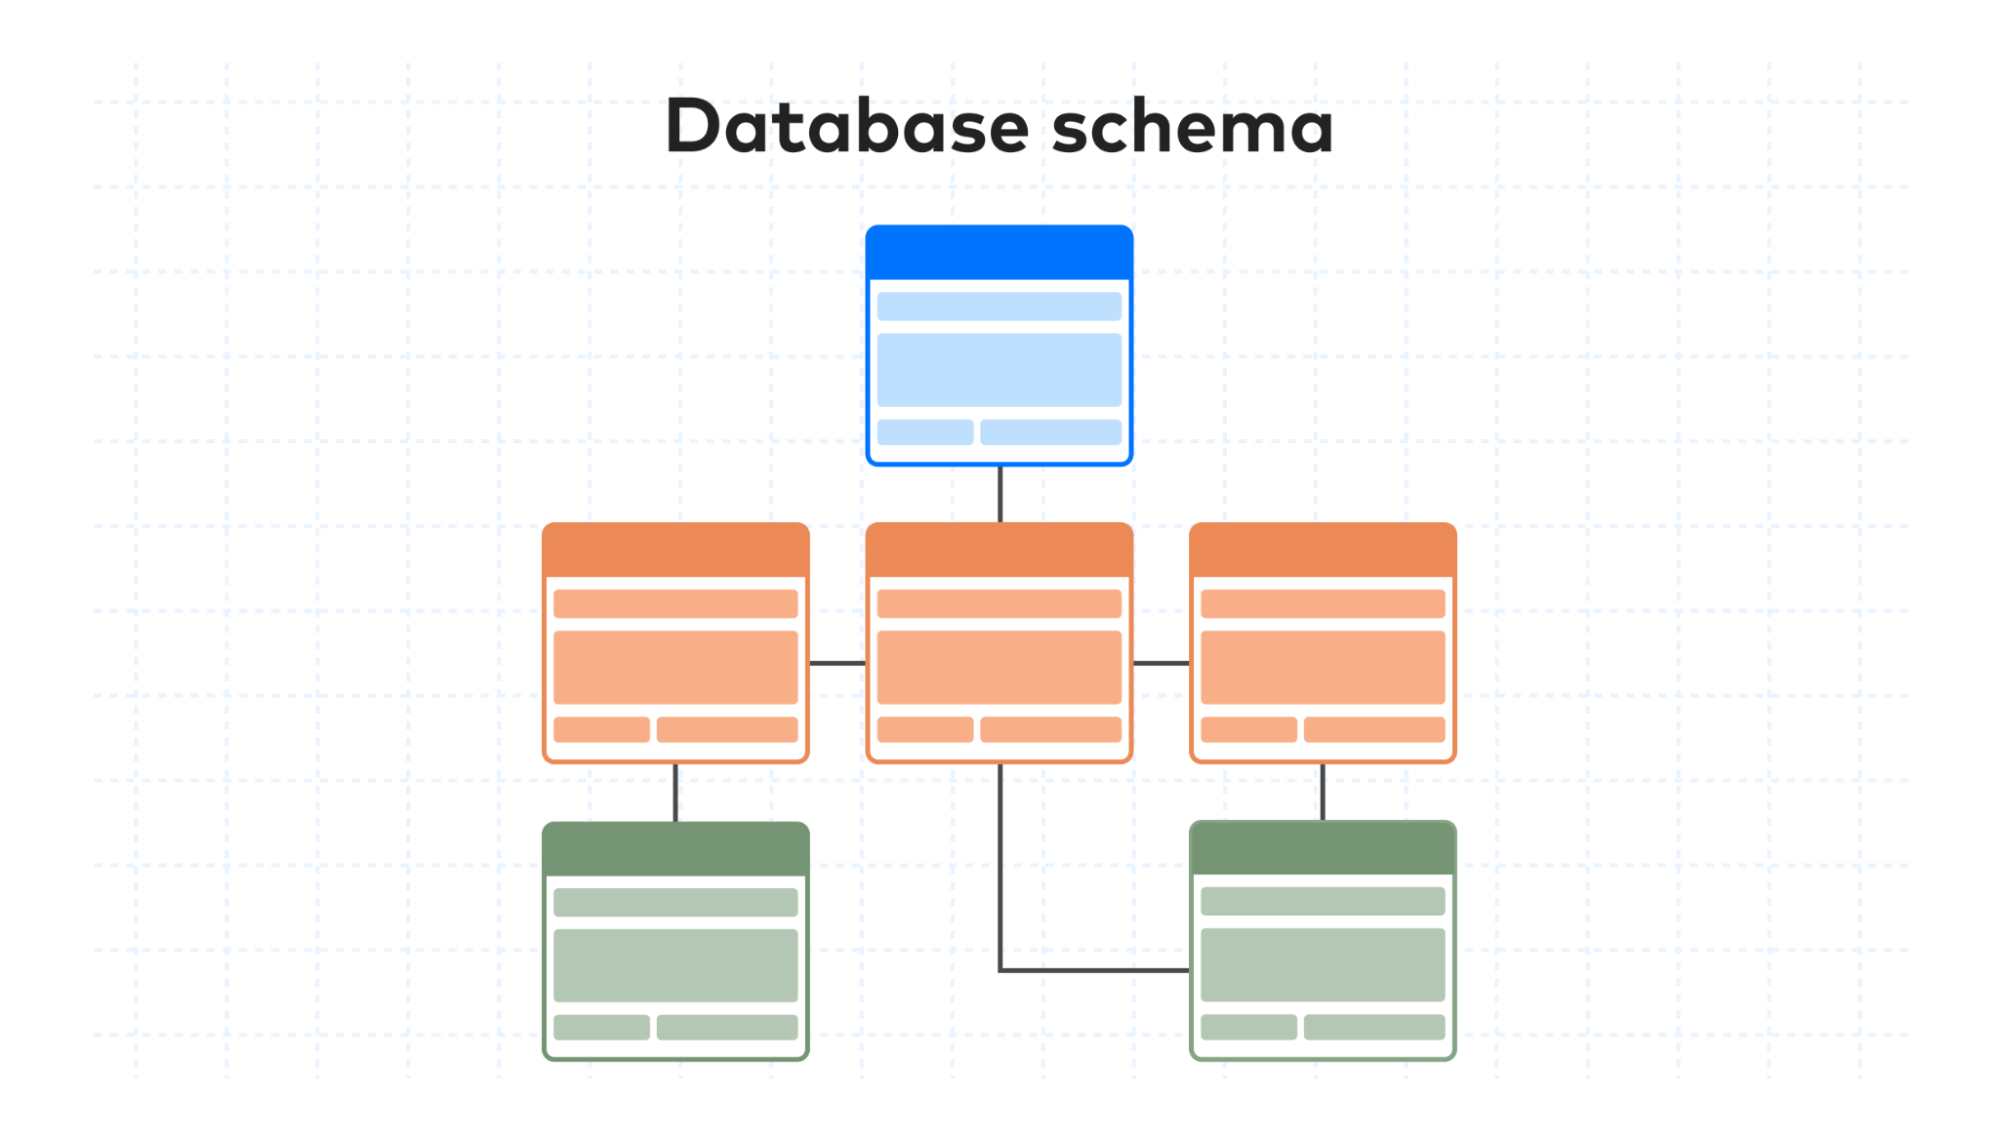
\includegraphics[width=0.9\textwidth]{img/database-schema.png}
    \end{figure}

\end{frame}


\begin{frame}{Schéma flexible}

    Donner example de schéma flexible

\end{frame}


\begin{frame}{Focus sur MongoDB}

\end{frame}

\begin{frame}{Étude de cas}

    Uber et MongoDB (gestion des trajets en temps réel).

    Problématique.
    Solution NoSQL choisie.
    Architecture mise en place.
    Résultats (performances, coûts).

\end{frame}

\begin{frame}[standout]

    Bases de données orientées colonne

\end{frame}

\begin{frame}{Caractéristiques des bases de données orientées colonne}

    \begin{definitionbox}
        Dans une base de données orientée colonne, les données sont stockées par \textbf{colonnes} plutôt que par lignes.

        Chaque ligne correspond à une clé unique, et les colonnes stockent des paires de \textbf{nom-colonne : valeur}, ce qui permet de regrouper des colonnes similaires pour une meilleure performance des requêtes en lecture.
    \end{definitionbox}

    \begin{noteblock}
        \begin{itemize}
            \item Optimisé pour les lectures massives sur des colonnes spécifiques.
            \item Très scalable et performant pour des requêtes analytiques.
        \end{itemize}
        $\hookrightarrow$ Idéal pour des applications nécessitant des analyses de grandes quantités de données.
    \end{noteblock}
\end{frame}

\begin{frame}{Bases de données orientées colonne}
    \begin{figure}[htb]
        \centering
        \begin{tikzpicture}
            \node[minimum width=3cm, minimum height=2cm] at (0, 0) {\includesvg[height=1.1cm]{img/db/cassandra.svg}};
            \node[minimum width=3cm, minimum height=2cm] at (4, 0) {\includesvg[height=0.9cm]{img/db/hbase.svg}};
            \node[minimum width=3cm, minimum height=2cm] at (0, -2) {\includesvg[height=0.7cm]{img/db/druid.svg}};
            \node[minimum width=3cm, minimum height=2cm] at (4, -2) {
\includegraphics[height=1.5cm]{img/db/scylla-db.png}};
            \node[minimum width=3cm, minimum height=2cm] at (0, -4) {
\includegraphics[height=1cm]{img/db/gcp-bigtable.png}};
            \node[minimum width=3cm, minimum height=2cm] at (4, -4) {
\includegraphics[height=1cm]{img/db/hypertable.png}};
        \end{tikzpicture}
    \end{figure}
\end{frame}

\begin{frame}{Exemple : distribution des données sur Cassandra}

    \begin{figure}
        \centering
        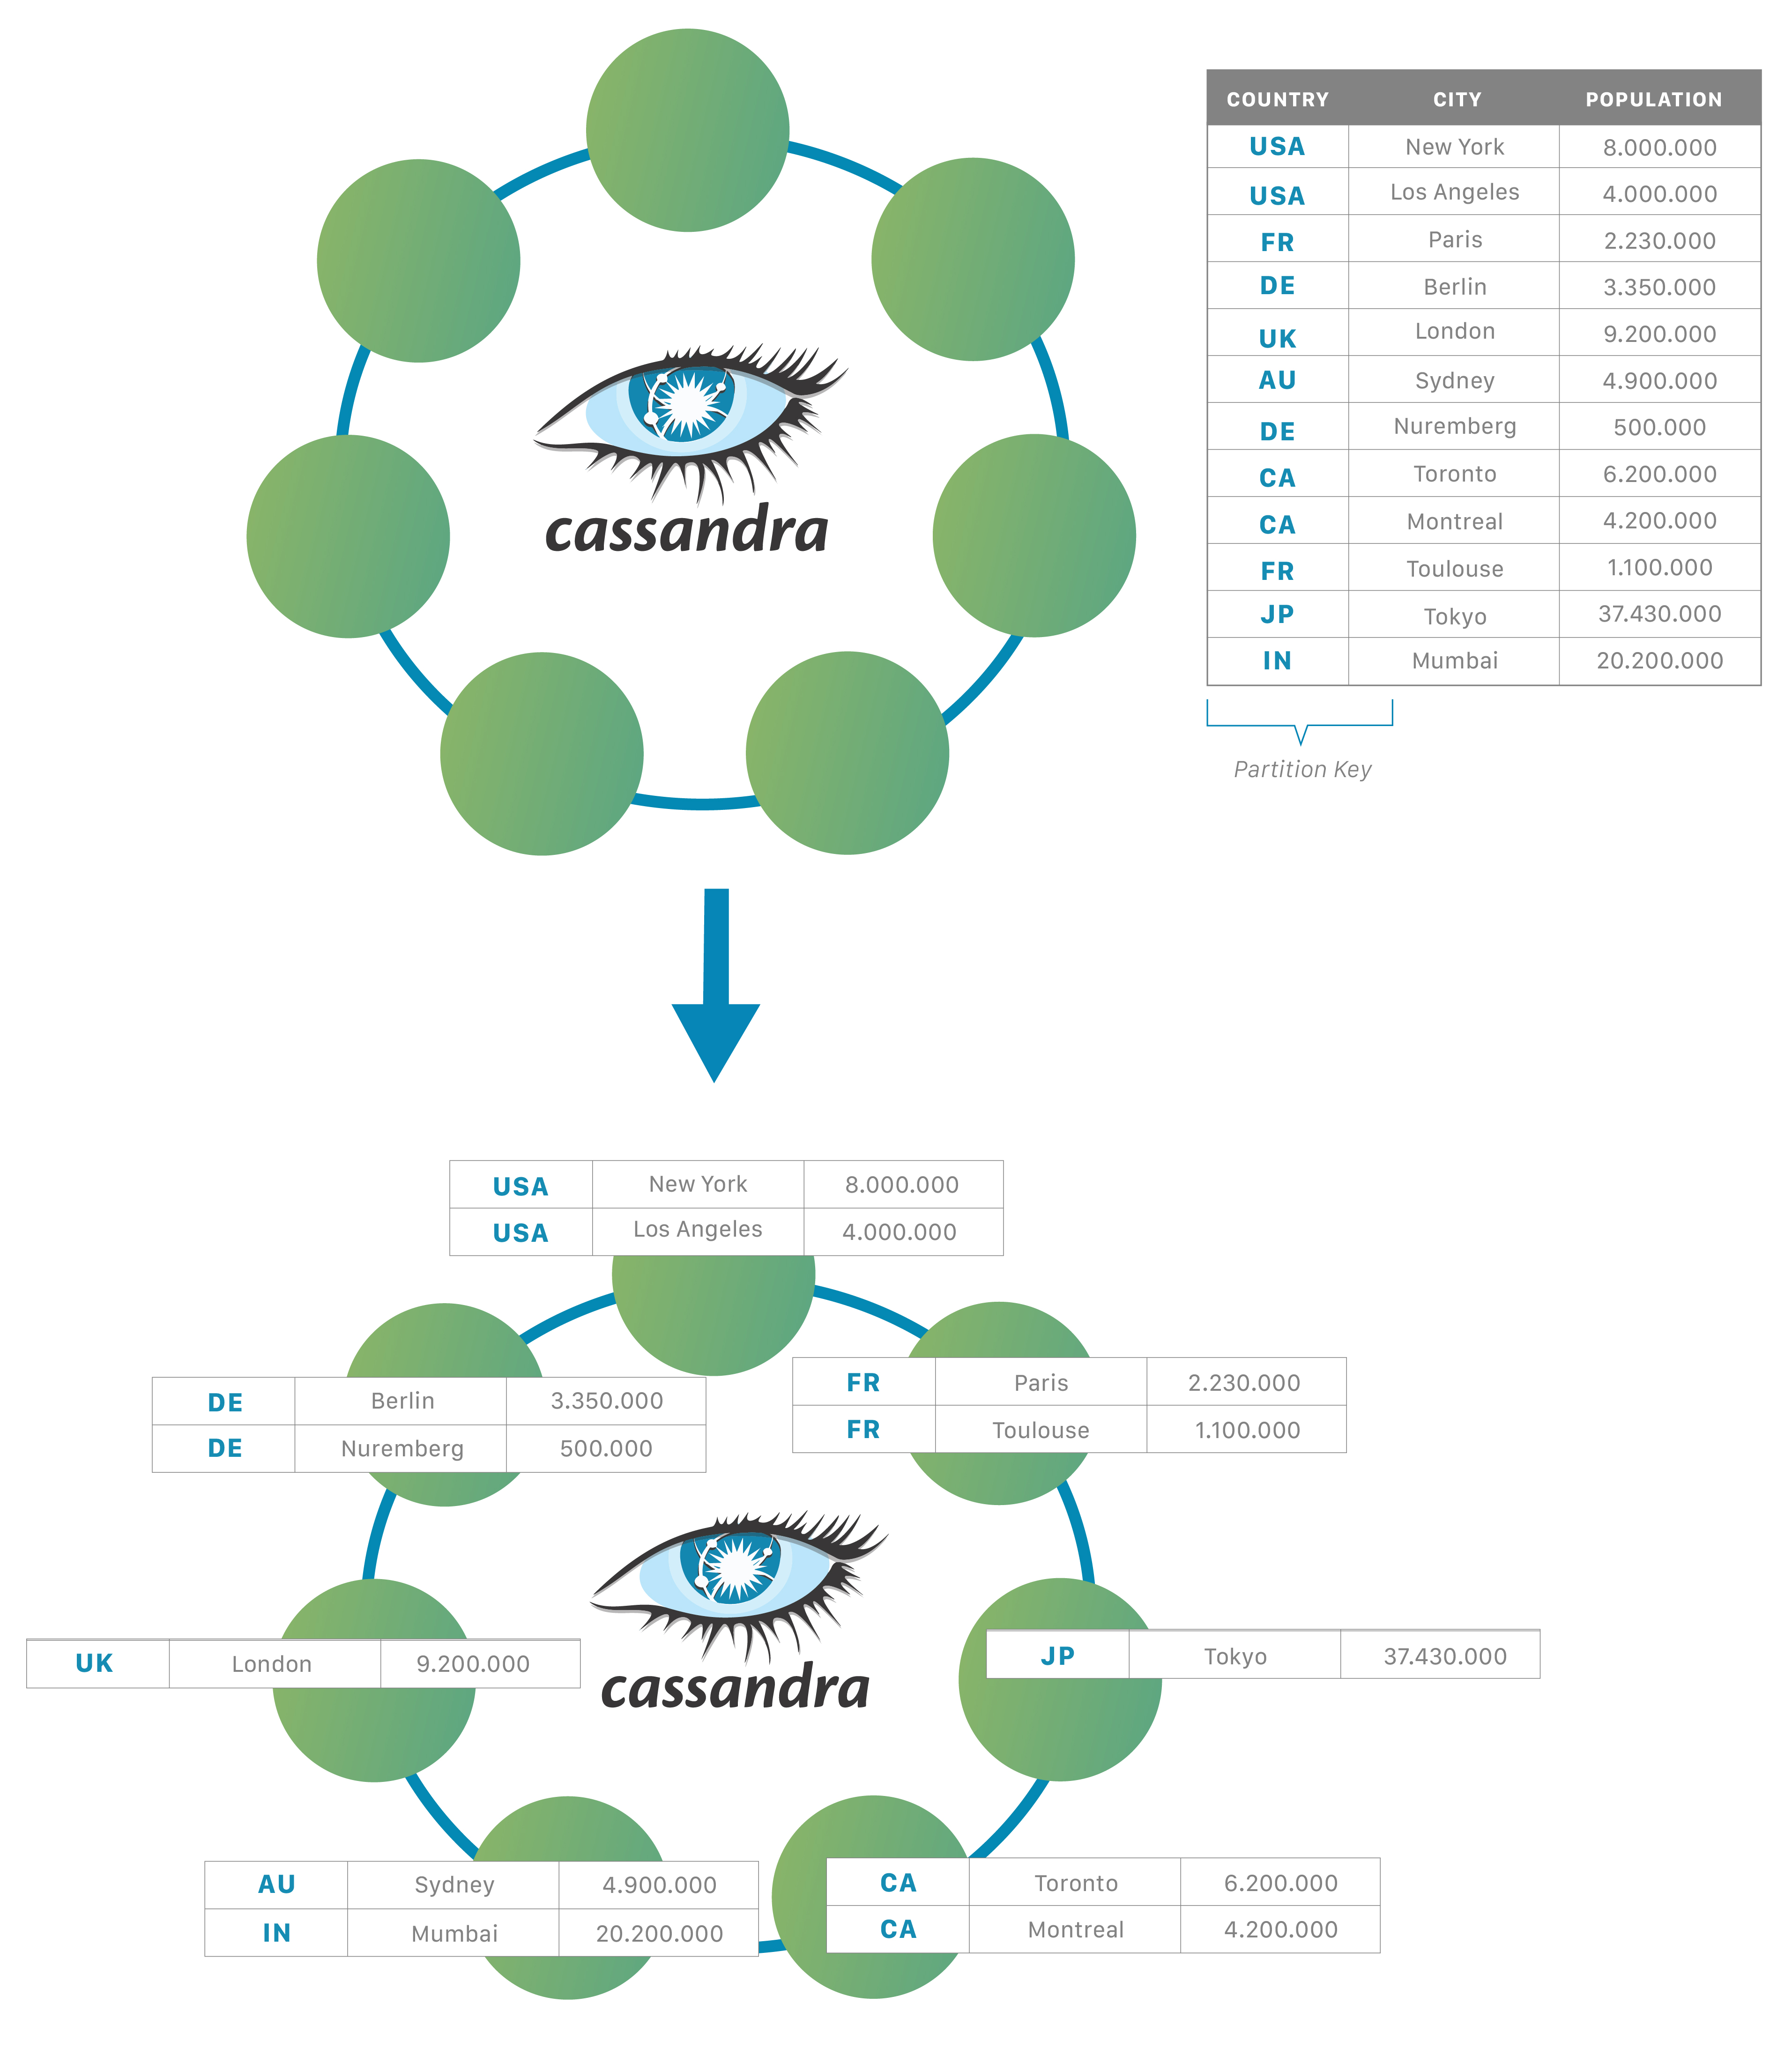
\includegraphics[width=0.8\textheight]{img/apache-cassandra-nodes.jpg}
    \end{figure}

\end{frame}

\begin{frame}{Cas d'usages des bases de données orientées colonne}

\begin{itemize}
    \item \textbf{Systèmes de gestion des données financières}\\
    $\hookrightarrow$ Permet d'extraire rapidement des colonnes spécifiques comme les prix ou les transactions sur de grands ensembles de données.
    \vspace{0.3cm}

    \item \textbf{Outils analytiques et de Big Data}\\
    $\hookrightarrow$ Optimisé pour les requêtes analytiques complexes sur des jeux de données massifs.
    \vspace{0.3cm}

    \item \textbf{Moteurs de recommandation}\\
    $\hookrightarrow$ Stocke des informations sur les utilisateurs et leurs préférences sous forme de colonnes, permettant une extraction rapide pour les recommandations en temps réel.
\end{itemize}
\end{frame}

\begin{frame}{Avantages et inconvénients des bases de données colonne}
\vfill
\prosbox{
    \textbf{Avantages}
    \begin{itemize}
        \item Très performant pour les requêtes en lecture sur des colonnes spécifiques.
        \item Scalabilité horizontale adaptée pour le traitement de données massives.
        \item Idéal pour des applications analytiques ou des systèmes OLAP.
    \end{itemize}
}
\vfill
\pause
\consbox{
    \textbf{Inconvénients}
    \begin{itemize}
        \item Moins efficace pour des écritures fréquentes ou des transactions complexes.
        \item Complexité accrue pour gérer les relations entre colonnes.
    \end{itemize}
}
\vfill
\end{frame}

\begin{frame}{Focus sur Apache Cassandra}

\end{frame}

\begin{frame}{Étude de cas}

    Netflix et Cassandra (scalabilité pour le streaming).

    Problématique.
    Solution NoSQL choisie.
    Architecture mise en place.
    Résultats (performances, coûts).

\end{frame}

\begin{frame}[standout]

    Bases de données orientées graphe

\end{frame}

\begin{frame}{Caractéristiques des bases de données graphe}

    \begin{definitionbox}
        Dans une base de données graphe, les données sont organisées en \textbf{nœuds}, \textbf{liens} et \textbf{propriétés} qui permettent de modéliser des relations complexes et dynamiques entre les entités. Les \textbf{nœuds} représentent les entités, les \textbf{liens} représentent les relations entre ces nœuds, et les \textbf{propriétés} fournissent des informations supplémentaires sur les nœuds et les liens.
    \end{definitionbox}

    \begin{noteblock}
        \begin{itemize}
            \item Représentation des relations complexes entre les données.
            \item Optimisé pour les requêtes de lecture et les opérations relationnelles.
        \end{itemize}
        % $\Longrightarrow$ Idéal pour des applications nécessitant des relations complexes et dynamiques entre les données.
        $\hookrightarrow$ Idéal pour des applications nécessitant des relations complexes et dynamiques entre les données.
    \end{noteblock}
\end{frame}

\begin{frame}{Bases de données graphe}
    \begin{figure}[htb]
        \centering
        \begin{tikzpicture}
            \node[minimum width=3cm, minimum height=2cm] at (0, 0) {\includesvg[height=1cm]{img/db/neo4j.svg}};
            \node[minimum width=3cm, minimum height=2cm] at (4, 0) {\includesvg[height=0.8cm]{img/db/arangodb.svg}};
            \node[minimum width=3cm, minimum height=2cm] at (0, -3) {
\includegraphics[height=1.3cm]{img/db/aws-neptune.png}};
            \node[minimum width=3cm, minimum height=2cm] at (4, -3) {\includesvg[height=1.3cm]{img/db/orientdb.svg}};
        \end{tikzpicture}
    \end{figure}
\end{frame}

\begin{frame}{Comment fonctionnent les bases de données graphe ?}

    \begin{figure}
        \centering
        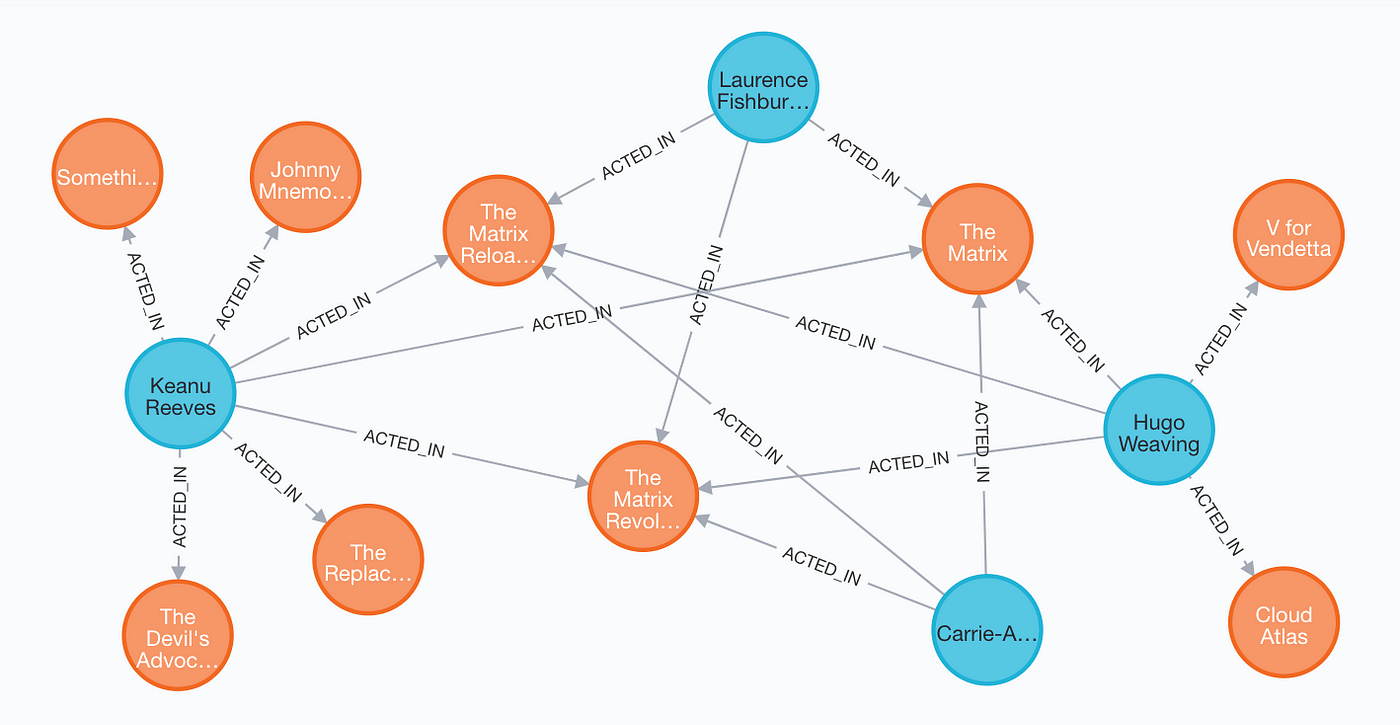
\includegraphics[width=0.8\textwidth]{img/neo4j-graph.png}
    \end{figure}

\end{frame}

\begin{frame}{Cas d'usages des bases de données graphe}

    \begin{itemize}
        \item \textbf{Réseaux sociaux}\\
        $\hookrightarrow$ Modélisation des relations entre utilisateurs, amis, groupes, et interactions pour des recommandations et des analyses sociales.
        \vspace{0.3cm}

        \item \textbf{Détection de fraude}\\
        $\hookrightarrow$ Analyse des connexions entre transactions et entités pour identifier des schémas de fraude ou des comportements suspects.
        \vspace{0.3cm}

        \item \textbf{Systèmes de recommandation}\\
        $\hookrightarrow$ Analyse des préférences des utilisateurs et des relations entre produits pour fournir des recommandations personnalisées.
        \vspace{0.3cm}

        \item \textbf{Gestion des réseaux de télécommunications}\\
        $\hookrightarrow$ Modélisation des réseaux de télécommunications et des relations entre équipements pour optimiser les performances et la maintenance.
    \end{itemize}
\end{frame}

\begin{frame}{Avantages et inconvénients des bases de données graphe}
    \vfill
    \prosbox{
        \textbf{Avantages}
        \begin{itemize}
            \item Excellente performance pour les requêtes impliquant des relations complexes.
            \item Flexibilité pour modéliser des structures de données dynamiques.
        \end{itemize}
    }
    \vfill
    \pause
    \consbox{
        \textbf{Inconvénients}
        \begin{itemize}
            \item Moins efficace pour les opérations non liées aux relations.
            \item Complexité accrue pour les utilisateurs non familiers avec la modélisation en graphe.
        \end{itemize}
    }
    \vfill
\end{frame}


\begin{frame}{Focus sur Neo4j}

\end{frame}

\begin{frame}{Étude de cas}

    LinkedIn et Neo4j (recommandations de connexions).

    Problématique.
    Solution NoSQL choisie.
    Architecture mise en place.
    Résultats (performances, coûts).

\end{frame}


% ------------------------------------------------------------------------------------------------------------------------------------------------------------------------

\begin{frame}{Retour sur le théorème CAP}

    Faire graphe et placer les différents systèmes (RDBMS, NoSQL, etc.)

\end{frame}

\begin{frame}{Retour sur le théorème CAP}

    \begin{figure}[htb]
        \resizebox{!}{0.85\textheight}{
        \begin{tikzpicture}
            % Circle 1: Consistency
            \draw[very thick, color=color-consistency, pattern=north east lines, pattern color=color-consistency] (0,0) circle (3cm);
            \node[fill=color-consistency, text=white, font=\bfseries, rounded corners] at (0,0.5) {Consistency};

            % Circle 2: Availability
            \draw[very thick, color=color-availability] (-2.1,-3.25) circle (3cm);
            \node[fill=color-availability, text=white, font=\bfseries, rounded corners] at (-2.75,-3.5) {Availability};

            % Circle 3: Partition Tolerance
            \draw[very thick, color=color-partition] (2.1,-3.25) circle (3cm);
            \node[fill=color-partition, text=white, font=\bfseries, rounded corners, align=left] at (2.75,-3.5) {Partition \\ tolerance};

            \node[fill=none, font=\bfseries, text=color-ca] (ca) at (-1.4,-1.5) {CA};
            \node[fill=none, font=\bfseries, text=color-cp] (cp) at (1.4,-1.5) {CP};
            \node[fill=none, font=\bfseries, text=color-ap] (ap) at (0,-3.7) {AP};

            % Unicorn
            \node[inner sep=0pt] (unicorn) at (0,-2.25) {
\includegraphics[width=1cm]{img/unicorn.png}};

            % Relationships
            % AP
            \node[yshift=-3.1cm] at (ap.south) {\includesvg[width=3cm]{img/db/cassandra.svg}};
            % CP
            \node[xshift=3.25cm, yshift=2.5cm] at (cp.east) {\includesvg[width=3cm]{img/db/mongodb.svg}};
            \node[xshift=4cm, yshift=1.2cm] at (cp.east) {\includesvg[width=3cm]{img/db/redis.svg}};
            % CA
            \node[xshift=-1.8cm, yshift=4.5cm] at (ca.west) {RDBMS};
            \node[xshift=-1.8cm, yshift=4.2cm] at (ca.west) {\includesvg[width=2cm]{img/db/postgresql.svg}};
            \node[xshift=-2.8cm, yshift=2.4cm] at (ca.west) {\includesvg[width=2cm]{img/db/mysql.svg}};
            \node[xshift=-3.5cm, yshift=1cm] at (ca.west) {\includesvg[width=2cm]{img/db/neo4j.svg}};
        \end{tikzpicture}
        }
    \end{figure}
\end{frame}

\begin{frame}{Performance}

    Faire un tableau comparatif des performances des différents types de bases de données NoSQL avec un exemple.

    Exemple : Quel est le revenu moyen des utilisateurs par pays ?

    SQLite (RDBMS) vs MongoDB (Document) vs Cassandra (Column) vs Neo4j (Graph)

\end{frame}

% Quiz

\begin{frame}[standout]

    Avez-vous été attentifs ?

    À vous de jouer !

\end{frame}

{
\setbeamercovered{transparent}

\begin{frame}{Q1}

    \textbf{Quels sont les quatre principaux types de bases de données NoSQL ?}

    \begin{itemize}
        \item \uncover<1>{\textcolor{kh-red}{Colonne, Clé-Valeur, XML, Graph}}
        \item \uncover<1>{\textcolor{kh-blue}{JSON, Colonne, Document, Graph}}
        \item \uncover<1>{\textcolor{kh-green}{Clé-Valeur, Table, Document, SQL}}
        \item \textbf<2>{\textcolor{kh-yellow}{Clé-Valeur, Colonne, Document, Graph}}
    \end{itemize}

\end{frame}

\begin{frame}{Q2}

    \textbf{Dans une base de données de type document, sous quelle forme les données sont-elles stockées ?}

    \begin{itemize}
        \item \uncover<1>{\textcolor{kh-red}{Clé-valeur}}
        \item \textbf<2>{\textcolor{kh-blue}{JSON ou BSON}}
        \item \uncover<1>{\textcolor{kh-green}{Table}}
        \item \uncover<1>{\textcolor{kh-yellow}{Colonne}}
    \end{itemize}

\end{frame}

\begin{frame}{Q3}

    \textbf{Quelle base de données NoSQL est conçue pour les requêtes de graphe complexe ?}

    \begin{itemize}
        \item \uncover<1>{\textcolor{kh-red}{Redis}}
        \item \uncover<1>{\textcolor{kh-blue}{Apache Cassandra}}
        \item \textbf<2>{\textcolor{kh-green}{Neo4j}}
        \item \uncover<1>{\textcolor{kh-yellow}{MongoDB}}
    \end{itemize}

\end{frame}

\begin{frame}{Q4}

    \textbf{Quelle base de données est plus adaptée pour un jeu vidéo ?}

    En tant que membre d'une équipe de développeurs de jeux, vous avez été chargé de concevoir un moyen de suivre les possessions des joueurs (achetées dans un catalogue, échangées entre joueurs ou via des récompenses). Les possessions sont classées en vêtements, outils, livres et pièces de monnaie. Les joueurs peuvent avoir un nombre illimité de possessions de n'importe quel type. Les joueurs peuvent rechercher d'autres joueurs possédant des types de possessions particuliers pour des échanges. Le concepteur du jeu informe qu'il y aura probablement de nouveaux types de possessions et de nouvelles façons de les acquérir à l'avenir. Quel type de base de données recommanderiez-vous d'utiliser ?

    \begin{itemize}
        \item \uncover<1>{\textcolor{kh-red}{Base de données transactionnelle}}
        \item \uncover<1>{\textcolor{kh-blue}{Base de données orientée colonne}}
        \item \textbf<2>{\textcolor{kh-green}{Base de données orientée document}}
        \item \uncover<1>{\textcolor{kh-yellow}{Base de données analytique}}
    \end{itemize}

\end{frame}

\begin{frame}{Q5}

    \textbf{Quelle base de données est plus adaptée pour un logiciel ?}

    Un développeur de logiciels vous demande conseil sur le stockage des données. Il dispose de centaines de milliers d'objets JSON de 1 Ko qui doivent être accessibles en moins d'une milliseconde si possible. Tous les objets sont référencés par une clé. Il n'est pas nécessaire de rechercher des valeurs dans le contenu de la structure JSON. Quel type de base de données NoSQL recommanderiez-vous ?

    \begin{itemize}
        \item \uncover<1>{\textcolor{kh-red}{Base de données orientée graphe}}
        \item \uncover<1>{\textcolor{kh-blue}{Base de données analytique}}
        \item \uncover<1>{\textcolor{kh-green}{Base de données orientée colonne}}
        \item \textbf<2>{\textcolor{kh-yellow}{Base de données clé-valeur}}
    \end{itemize}

\end{frame}

\begin{frame}{Q6}

    \textbf{Quelle base de données est plus adaptée pour un logiciel ?}

    Une développeuse de logiciels vous demande conseil sur le stockage de données. Il a des centaines de milliers d'objets JSON de 10 Ko qui doivent pouvoir être recherchés par la plupart des attributs de la structure JSON. Quel type de base de données NoSQL recommanderiez-vous ?

    \begin{itemize}
        \item \textbf<2>{\textcolor{kh-red}{Base de données orientée document}}
        \item \uncover<1>{\textcolor{kh-blue}{Base de données orientée colonne}}
        \item \uncover<1>{\textcolor{kh-green}{Base de données analytique}}
        \item \uncover<1>{\textcolor{kh-yellow}{Base de données clé-valeur}}
    \end{itemize}

\end{frame}

%\begin{frame}{Q7}
%
%    \textbf{Une programmeuse conçoit une base de données pour prendre en charge les requêtes ad hoc. Quel type de schéma de données est-il susceptible d'utiliser ?}
%
%    \textit{Une requête ad hoc est une requête qui est créée pour répondre à un besoin d'information spécifique, souvent de manière ponctuelle, et qui n'est pas prévue ou récurrente dans les opérations normales de la base de données.}
%
%    \begin{itemize}
%        \item \uncover<1>{\textcolor{kh-red}{Online Transaction Processing (OLTP)}}
%        \item \textbf<2>{\textcolor{kh-blue}{Online Analytical Processing (OLAP)}}
%        \item \uncover<1>{\textcolor{kh-green}{Schéma normalisé}}
%        \item \uncover<1>{\textcolor{kh-yellow}{Schéma Dénormalisé}}
%        \item \uncover<1>{\textcolor{kh-teal}{Graphe de connaissances}}
%    \end{itemize}
%
%\end{frame}

%\begin{frame}{Q8}
%
%    \textbf{}
%
%    \begin{itemize}
%        \item \uncover<1>{\textcolor{kh-red}{}}
%        \item \uncover<1>{\textcolor{kh-blue}{}}
%        \item \textbf<2>{\textcolor{kh-green}{}}
%        \item \uncover<1>{\textcolor{kh-yellow}{}}
%    \end{itemize}
%
%\end{frame}
%
%\begin{frame}{Q9}
%
%    \textbf{}
%
%    \begin{itemize}
%        \item \uncover<1>{\textcolor{kh-red}{}}
%        \item \uncover<1>{\textcolor{kh-blue}{}}
%        \item \textbf<2>{\textcolor{kh-green}{}}
%        \item \uncover<1>{\textcolor{kh-yellow}{}}
%    \end{itemize}
%
%\end{frame}
%
%\begin{frame}{Q10}
%
%    \textbf{}
%
%    \begin{itemize}
%        \item \uncover<1>{\textcolor{kh-red}{}}
%        \item \uncover<1>{\textcolor{kh-blue}{}}
%        \item \textbf<2>{\textcolor{kh-green}{}}
%        \item \uncover<1>{\textcolor{kh-yellow}{}}
%    \end{itemize}
%
%\end{frame}

}

